%!TEX root = ../thesis.tex

\graphicspath{{Chapter1/Figures/}{Chapter1/Tables/}{Chapter1/Charts/}}

\chapter{Introduction}

\section{Research Context} %Section - 1.1 
There are many critical decisions that face software development practitioners throughout the development lifecycle, ultimately contributing to the success or failure of a project. These decisions, broadly, fall under the categories of Process, Technology, or People \citep{nasir2011critical}. Decisions in the Process category are those such as the choice of development methodology \citep{chow2008survey, vijayasarathy2016choice}, development standards \citep{rainer2002key}, or the decision to invest in test automation to achieve shorter testing cycles \citep{lewis2016software}. Technology decisions can vary from questions of what hardware or programming languages to use for development to the selection of tools that development teams should employ \citep{scheer2000enterprise, ray2017survey, chen2018gflink, eichhorn2018comparative}. Finally, the People category of decisions focuses on issues such as the resourcing and staffing of software development project teams and how those teams fit into the wider organisation \citep{krishnan1998role, andrejczuk2017synergistic, alfayez2018exploratory}.

Each of these categories of decisions has seen a great deal of academic research. In the Process category Kuhrmann et al. \citep{kuhrmann2015software} conducted a mapping study of the field of software process improvement, finding 635 publications over the past 25 years. To give a flavour of these studies, some investigate how greater adherence to established software process models such as CMM \citep{paulk1993capability} or ISO \citep{ISO15504} can result in better quality \citep{harter2012does, abrahamsson2013measuring}. Others are case studies into how organisations manage adoption of process models with refinements proposed for particular contexts such as small or medium enterprises \citep{balla2001quality, sulayman2012software}. Research in the Technology category is extremely broad covering topics such as the suitability of particular technologies for a given use \citep{sharp2003evaluating, baker2006real}, the security implications of using a given technology stack \citep{mirheidari2012two, choukse2012developing, gangwar2014web}, or studies of the tools that can be used to facilitate team communication in a global context \citep{portillo2012tools}. Finally, in the People category the research, again broad and diverse, can vary from a study of what motivates open-source software contributors through to the impact of team size or team diversity on team performance \citep{hoch2010most, von2012carrots}. 

Of these three categories, 'People' decisions are established to have the greatest impact on development team productivity \citep{trendowicz2009factors} and critical success factors for software development projects are, by far, more likely to be in the realm of people factors \citep{boehm1978characteristics, onoue2018human}. Software development is intrinsically a human activity and a more people-oriented approach is in the ascendency evident in, amongst other things, increasing adoption of agile methodologies \citep{pirzadeh2010human}.

Nasir et al. \citep{nasir2011critical} conducted an extensive literature survey of the critical success factors that impact software projects finding that in the People category some of the most cited project success factors, based on industrial case studies as well as surveys, relate specifically to the composition of the software development team \citep{schmidt2001identifying, sauer2003state, humphrey2005big, kappelman2006early, glass2006standish}. This is pertinent because within most real world software development projects those 'people' decisions - for instance the composition of individual development teams - can be made by managers who are not particularly senior and, indeed, often with input from individual developers. By contrast, location strategies or project budgets are often dictated by senior management with little or no influence from those lower in the management chain and are therefore within the sphere of influence of significantly fewer practitioners. When considering decentralised volunteer-based Free Libre Open-Source (FLOSS) projects, it is also true that, beyond the composition of the software development team, there can be limited tools with which stakeholders can influence the success or failure of a project \citep{schweik2008brooks}.

In the context of this research, team size is a measure of the number of developers that modify a project source code. Within that same context team stability is taken as function of the cumulative time that each developer has worked with their fellow team members. Within the 'People' category of research there is an extensive body of work that empirically proves that team size and stability are linked to specific external attributes of the produced software such as fault-proneness as well as more general aspects such as project success rates and team productivity. As will be detailed in the next chapter titled 'Related Work', earlier research established that smaller or more stable development teams are more productive, produce less fault-prone software, and have higher levels of stakeholder satisfaction.  Much of this research has been motivated, at least in part, to help inform practitioners on how to compose their own development teams so that the associated risks can be limited as far as practicable, recognising that team composition is one of the few levers within the grasp of management to strongly influence project outcomes. 

The research asserts that new insights can be gained into how team size and stability impact the produced software by measuring the internal attributes of the software instead of the more traditional approach of measuring its external attributes. Through this approach practitioners can form a more complete picture to inform decision-making. Uniquely, this also enables practitioners to measure and monitor key indicators, taking remedial action at earlier stages in the development lifecycle.

\section{Team Size and Stability in the Literature} %Section - 1.2
In 1974 Brooks, in his popular book 'The Mythical Man Month', stated that adding additional developers to a project can result in a loss of productivity due to the exponential difficulties involved in maintaining effective communication within a larger team \citep{brooks1986mythical}. In 2000, Raymond, in his book 'The Cathedral and the Bazaar', asserted that in open-source software development larger development teams are more effective at identifying and resolving bugs, leading to less fault-prone software. Raymond termed this 'Linus Law' named after the lead linux developer. In contrast to both Brooks and Linus law is the 'Core Team principle' that states that the size of a team should not have an impact on the success of the project as core development groups are always small. For researchers or practitioners, attempting to navigate these somewhat conflicting principles to understand which factors will win out is no easy task \citep{schweik2008brooks}. 

Greater consensus is evident when reviewing the literature around team stability - a significantly smaller body of work - which agrees that more stable teams produce less fault-prone software. One particularly stark observation was that as team stability increased by 50\% defects decreased by 19\% \citep{huckman2009team}.

Questions of how development team size and stability impact fault-proneness is also very much at the forefront of practitioner minds. Many practitioners have taken the time to present their evidence and document their experience around these two particular strands in whitepapers and blog posts, generally agreeing with the academic research - some through empirical means \citep{macheronne2013critical, mcconnell2017less}, others purely anecdotal \citep{miller2006critical, erickson2012are, meccia2015critical, plowman2015seven} - that smaller, more stable teams produce less fault-prone software. This is covered in more detail in the 'Related Work' chapter.

Interest in fault-proneness is not without good reason. There are numerous examples of software faults causing governmental or corporate institutions severe reputational damage. Knight Capital is oft-cited as an example of how costly fault-proneness can be after a defect in their order routing software caused a \$465 million trading loss \citep{sec2013}. Behind the headline grabbing incidents is a more pervasive issue throughout the industry. A 2013 Cambridge University study estimated that software bugs cost the global economy \$312 billion annually \citep{britton2013reversible}. That same study found that developers spend half their time debugging software.

However, fault-proneness is not the only aspect that of concern to stakeholders. Maintainability has also seen significant research activity. This refers to the ease with which a software system or component can be modified to correct faults, improve performance or other attributes, or adapt to a changed environment \citep{radatz1990ieee}. ISO 9126 states that maintainability is comprised of four sub-attributes - analysability, changeability, stability, and testability \citep{ISO9126}. Highly analysable software requires lower effort to investigate and understand sections of the codebase in order to remediate defects or to adapt the codebase to new requirements. Similarly, high levels of changeability require less effort to implement changes in the codebase. Stability implies a lower likelihood that making changes to the software may have unintended negative impacts. Finally, testability is a measure of the effort required to adequately test software. Taken together, a codebase exhibiting high-levels of each of these sub-attributes of maintainability support a more adaptable business against a backdrop of an oft-changing competitive landscape. 

It is of crucial importance that researchers and practitioners alike understand the impact of any factors that can have a material impact on the maintainability of software. The focus of this thesis is to add evidence and insights on how development team size and team stability play a role as factors in the maintainability of produced software.

\section{Internal and external factors in the literature} %Section - 1.3
Figure~\ref{fig:PeopleInternalExternal} depicts, at a very high-level, the relationship that existing literature has established between the internal structural attributes of software and its maintainability.

Prior research has focused on establishing mathematical models that describe the impact of the internal attributes of software on its external attributes including maintainability. In these models the internal attributes are the independent variables while the external attributes are the dependent variables. Broadly, these models establish that lower coupling and complexity are more favourable structural properties, leading to lower fault proneness and greater maintainability. Conversely, higher cohesion and modularity are associated with that same favourable outcome of lower fault proneness and greater maintainability. Tables 2.2 and 2.5 neatly summarise these relationships which will be detailed in the next chapter titled 'Related Work'. 

This work takes an alternative yet complementary approach to the existing body of research. The research questions in this thesis centre around establishing the impact of team composition on the internal attributes of software, essentially treating the team factors as the independent variables and the internal attributes as the dependent variables. Using the aforementioned models from existing research, these observations are subsequently used to deduce the likely impact of these team factors on maintainability. Given the breadth of the work modelling the impact of internal attributes on external attributes, this could be used to apply the observations in this research to other external attributes beyond maintainability.

\begin{figure}[htbp!] 
\centering    
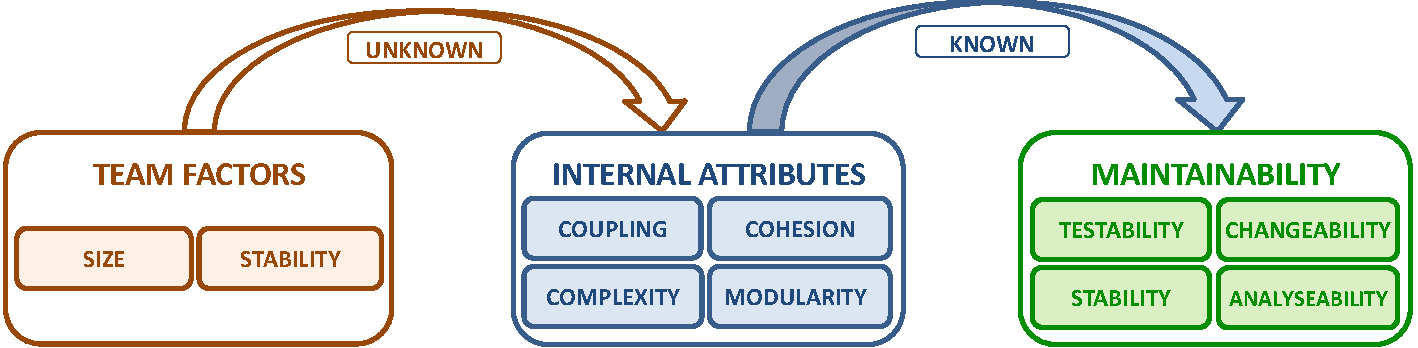
\includegraphics[width=1.0\textwidth]{PeopleInternalExternal.pdf}
\caption[The impact of 'people' factors on internal and external attributes of software]{The impact of 'people' factors on internal and external attributes of software}
\label{fig:PeopleInternalExternal}
\end{figure}

\section{Research Problem and Approach} %Section - 1.4
Effective teams are crucial to the success of organisations, especially in environments that require teams to be constantly created and dismantled as is the case in software development \citep{andrejczuk2017synergistic}. When organisations are tasked with delivering business critical software, they are often faced with multiple options to resource the project. These options could include externally recruiting a number of developers from the market and forming a new team or alternatively seconding an existing stable team comprised of developers with prior experience of working together - either from within the organisation or from an external vendor. 

After reviewing the existing research which does correlate team size and stability with fault-proneness it is notable that no insight is gained into how the internal attributes of software - such as coupling, cohesion, complexity and modularity - are impacted through these aspects of team composition. Given that the internal attributes of software essentially drive the aforementioned externally observable attributes (amongst others), it follows that, by all rights, this should be a crucial area of study, through which researchers can drive a deeper understanding of the impact of team composition on the aspects of stakeholder relevance such as fault-proneness and maintainability. The current state of research leaves academics and practitioners alike to draw their own conclusions on what changed internal attributes could be driving any externally observable attributes - and whether, for example, increased likelihood of fault-proneness could be observed at an earlier stage in the development lifecycle at the code level and subsequently mitigated.  As Fenton rightly points out, practitioners are accustomed to measuring and monitoring internal attributes throughout the development process, and hence would be well placed to monitor and mitigate risks if they were broadly observable \citep{fenton2014software}.

In order to qualitatively or quantitatively assess the negative effect of inappropriately sized or unstable teams, it is essential to analyse the impact that team size and stability have on the sub-attributes of maintainability. Such research is essential to providing practitioners with the requisite insights to inform their decisions around team composition. While existing research informs us that more stable development teams produce less fault-proneness, understanding the impact on the analysability, changeability, testability and stability of the software would enable practitioners to forecast how team stability would impact the maintainability phase of the project. This would empower practitioners to make team composition decisions that are more likely to be aligned with business goals and increase the likelihood of project success. 

The empirical approach of this thesis is to measure the impact of team size and stability on the internal attributes of a software system that, in turn, have a proven impact on its maintainability. This is illustrated by Figure~\ref{fig:PeopleInternalExternal}: by measuring the impact that these factors have on the internal attributes of software, this work provides a indirect link between the people factors and the maintainability of such a system. The primary contribution of this thesis is to add to the existing body of work and to add evidence in the form of trends, correlations and models describing the relationship between team size and team stability with the produced software's internal attributes, complementing the previously established trends relating internal and external attributes as summarised in Table ~\ref{tab:PriorArtSummary} and discussed in detail in 'Related Work'.  

This research draws upon a formally popular FLOSS 'forge' - a centralised online system with tools to enable distributed development teams to work together - to provide a data set which can be mined for observations to drive the empirical work in this thesis.

\begin{table}
\captionof{table}{Summary of the relationship between structural attributes and the externally observable attributes of software, as established in prior research.}
\begin{tabular}
 \centering
 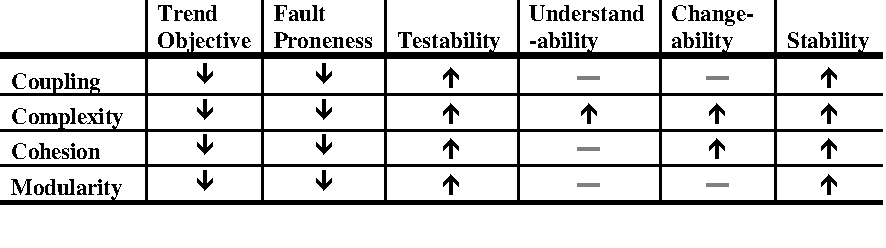
\includegraphics{PriorArtSummary.pdf}
 \label{tab:PriorArtSummary}
\end{tabular}
\end{table}
\section{Research Questions and Hypotheses} %Section - 1.5
Based on the survey of the related literature, the research questions focus on the two strands highlighted in the previously stated research problem. For each research question the null and alternative hypotheses are stated below.

\begin{itemize}
\item  \textbf{RQ1} \textit{What is the impact of development team size on the internal structural attributes of software projects and what are the implications on its maintainability?}
\begin{itemize}
\item \textbf{H0,1} \textit{Development team size does not impact the coupling, complexity, cohesion or modularity of the produced software.} Naturally the default starting position is to hypothesize that there is no relationship between team size and the structural attributes of software. 
\item \textbf{H1,1.1} \textit{Larger development teams produce software which exhibits greater coupling and complexity and lower cohesion and modularity when compared to that produced by smaller development teams.} Given existing research detailing the challenges that larger teams face in communication \citep{brooks1986mythical} and given the body of empirical research that finds that larger teams produce more fault prone software \citep{weyuker2008too, nagappan2008influence, meneely2009secure, foucault2015usefulness}, it follows that a reasonable hypothesis is that the internal structural attributes of the software produced by such a team will trend in a direction that is consistent with increasing fault-proneness; namely greater coupling and complexity, and lower cohesion and modularity. As both Linus law and the Core Team principle indicate the presence of forces that may ultimately work in favour of larger teams, such a hypothesis can only be proposed cautiously.
\item \textbf{H1,1.2} \textit{Larger development teams will produce less maintainable software when compared to that produced by smaller development teams.} As discussed in 'Related Work' in detail, cohesion is correlated with testability \citep{badri2011empirical} and analysability \citep{boehm1978characteristics} while coupling and complexity have been negatively correlated with stability \citep{elish2003investigation}. Given the previous hypothesis (H1,1.1) that larger teams will produce software which exhibits greater coupling and complexity and lower cohesion and modularity, the hypothesis follows that maintainability will likely deteriorate.
\end{itemize}
\item \textbf{RQ2} \textit{What is the impact of the development team stability on the internal structural metrics of coupling, cohesion, complexity, and modularity of software projects and what are the implications on its maintainability?}
\begin{itemize}
\item \textbf{H0,2} \textit{Development team stability does not impact the coupling, complexity, cohesion or modularity of the produced software.} Again, here the default starting position is to hypothesize that there is no relationship between team stability and the structural attributes of the software produced by that team. 
\item \textbf{H1,2.1} \textit{Less stable development teams produce software which exhibits greater coupling and complexity and lower cohesion and modularity when compared to more stable development teams.} Similarly to larger development teams, existing research shows that less stable teams also produce more fault-prone software and provide lower client satisfaction levels \citep{huckman2009team, gardner2012dynamically}. Naturally, this leads to a similar hypothesis to H1,1.1 that less stable teams will produce internal structural attributes which trend in a direction counter to the objective; namely greater coupling and complexity and lower cohesion and modularity.
\item \textbf{H1,2.2} \textit{Less stable development teams will produce less maintainable software when compared to more stable development teams.} Following a similar rationale to that expressed H1.1.2, given the hypothesis that less stable teams will produce software which exhibits greater coupling and complexity and lower cohesion and modularity, it follows that maintainability is hypothesised to deteriorate.
\end{itemize}
\end{itemize}

\section{Research Goals and Objectives} %Section - 1.6
The research questions and the related hypotheses are connected, in logical order, to the research goals. In the section below, each goal is formulated with its own rationale which is further elaborated on with a series of objectives, each justified by a rationale.

\begin{itemize}
\item  \textbf{Goal 1} \textit{To establish the impact of team size on the internal attributes of software and deduce the likely impact to maintainability.} 
This research goal is to conduct an analysis on the impact of team size on the structural metrics of software as a pathway to drawing insights into how this factor impacts the externally observable attributes of software. Within this overarching goal there are several objectives that facilitate a deeper knowledge of the underlying trends that impact structural metrics as precursor to formulating a credible methodology to execute the team size analysis.
\begin{itemize}
\item \textbf{Objective 1,1} Observe structural metrics trends throughout the evolution of software projects. As a codebase undergoes development iterations, increasing in functional complexity and code volume, the progression of the structural metrics exhibit trends which are necessarily of significance to any further analysis. 
\item \textbf{Objective 1,2} Control for confounding factors. These are factors that influence both the dependent and independent variables within a model causing a spurious association to be drawn. These factors can pose a significant threat to validity. For this reason, this objective aims to devise and execute an analytical approach to control for these confounding factors in order to ascertain the impact of team size alone.
\item \textbf{Objective 1,3} Formulate a definition of the software development team which enables its size to be observed through mining software repositories and analyse structural metrics across a sample data set to observe the impact of team size on the structural attributes of software. This objective goes to the heart of answering the first research question - RQ1.
\item \textbf{Objective 1,4} Deduce the likely result that the impact from team size on the structural metrics on software will have on the four sub-attributes of maintainability; changeability complexity, testability and analysability. This is to be done by referencing the relationships established in prior research between the internal and the external attributes of software. Once the impact of development team size on the structural metrics of a codebase is observed, the focus shifts to deducing the impact that this will have on the external attributes of the software.
\end{itemize}
\item  \textbf{Goal 2} \textit{To establish the impact of team stability on the internal attributes of software and deduce the likely impact to maintainability.}
\begin{itemize}
\item \textbf{Objective 2,1} From the prior research identify the pitfalls that exist in mining software repositories, how they apply to team stability analysis, and how they can be mitigated. Two challenges exist when conducting committer collaboration analysis in team stability analysis. The first is the effect that forking can have on the validity of results. Forking refers to the process of creating an alternate and independent software development stream from an existing project. As forked projects can retain the revision history of its parent, without proper identification and treatment, they can appear to be two independent projects with each set of authors contributing twice. The second challenge concerns tracking users throughout a forge - a task made complex by the fact that users often use subtly different identifiers through a project or while traversing a forge. These challenges should be met to ensure that they do not pose a significant threat to the validity of this research.
\item \textbf{Objective 2,2} Formulate a definition of the software development team stability and analyse structural metrics across a sample data set to observe the impact of team stability on the structural attributes of software. A nuanced approach is necessary to distinguish between team stability accrued through the course of a project and that stability that comes from the team remaining stable through the course of multiple projects. This objective drives towards an answer to the second research question - RQ2.
\item \textbf{Objective 2,3} Deduce the likely result that the impact from team stability on the structural metrics on software will have on the four sub-attributes of maintainability; changeability complexity, testability, analysability. Again, this is to be done by referencing the relationships established in prior research between the internal and the external attributes of software. Mirroring objective 1,4 concludes the answer to the second research question.
\end{itemize}
\end{itemize}

\begin{table}
\captionof{table}{A summary of the research questions, hypotheses, goals and objectives of this research.}
\begin{tabular}
 \centering 
 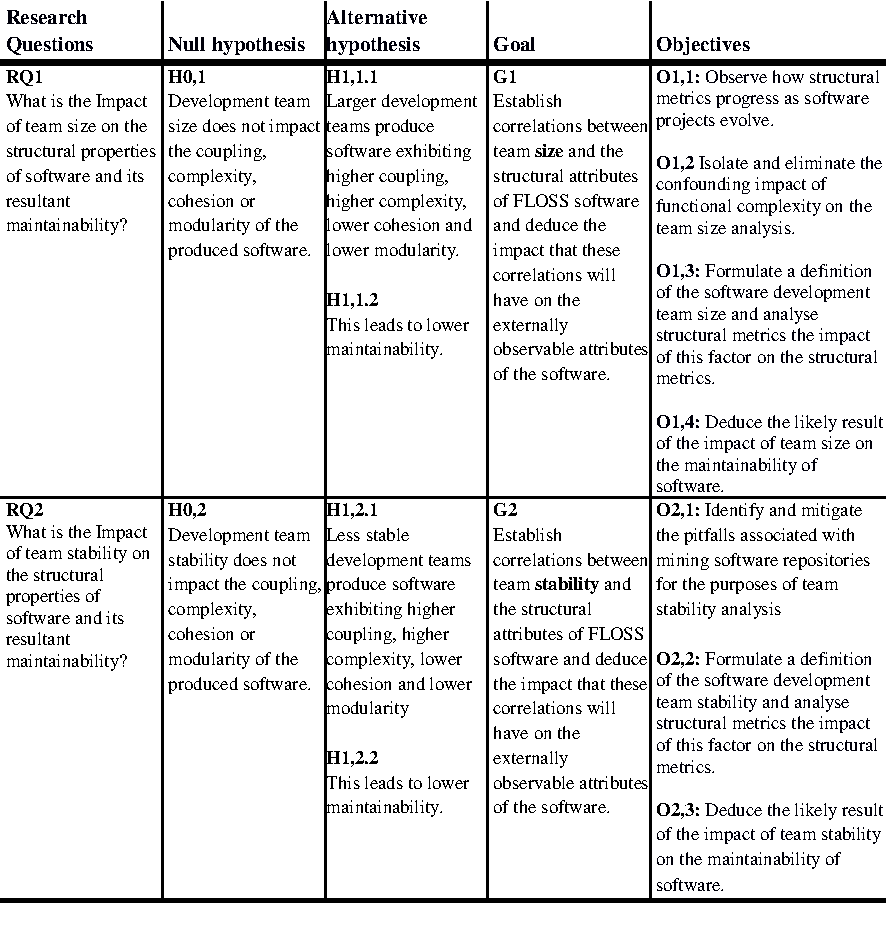
\includegraphics{ResearchSummary.pdf}
 \label{tab:researchSummary}
\end{tabular}
\end{table}

\section{Thesis Contribution} %Section - 1.7
Two main contributions to the state of the art can be identified within this thesis:

\begin{itemize}
\item \textbf{Advanced methodology to measure team size and stability:} This thesis presents an alternative approach to measuring the impact of team composition on external attributes by directly measuring the impact on its internal attributes and leveraging established research to deduce the ultimate impact on its external attributes. The impact of team size and stability on maintainability is studied through the GoogleCode forge and, in the process, numerous practical difficulties involved in mining a large and diverse forge are solved. In particular, this work identifies, quantifies and mitigates the previously undocumented and significant threat that forking can pose to the accuracy of forge analysis.

\item \textbf{Impact of team size and stability on internal structural attributes:} A clear relationship is established between team size and stability on the internal structural attributes of software. This research concludes that those projects developed by smaller or more stable teams exhibit lower levels of coupling and inheritance complexity and higher levels of cohesion and modularity. In addition to the observed trends, the state of the art is furthered through the proposal of two new measures to capture team stability, distinguishing between stability that accumulates as a team remains unchanged across projects and the stability which accumulates through the lifespan of an individual project through the collaboration of team members.
\end{itemize}

\section{Intended Audience} %Section - 1.8
This research is intended for both the research and practitioner communities. This thesis complements the existing body of research which correlates the internal attributes of software with observed external attributes by specifically studying the impact of team composition on these internal attributes. Researchers with an interest in relating software metrics to measures of stakeholder interest will find relevance in this work. It is also intended for this work to be of value to those practitioners in the field of software development. It is the intention of this thesis to contribute towards more informed practitioner decision-making around development team composition - particularly at the middle-management level. Furthermore, practically oriented observations of the impact of sub-optimal team composition, which can be monitored through static analysis of software, may find interest in the developer community.

\section{Thesis Structure} %Section - 1.9
The remainder of this thesis is arranged over five chapters as described below and illustrated in Figure ~\ref{fig:ThesisOverview}.

\textbf{Chapter 2. Related Work} Prior research is documented in three distinct fields. Firstly, a survey is conducted for previous research that establishes correlations between the development team's size and stability against attributes of stakeholder importance such as fault-proneness and team productivity. Secondly, a survey is carried out in the established field of mining software repositories and a sampling of research that employs mining techniques to observe changes in the properties of software is discussed. Finally, software metrics are considered with a focus on structural metrics and how they are interpreted and correlated with externally observable attributes of software such as maintainability.
\newline
\newline
\textbf{Chapter 3. Methodology} In this chapter the methodological approach to this research is detailed. Existing mining tools are surveyed and the mining toolchain that underpins this research will be discussed in depth. Metrics suites are also surveyed and justification is provided for the choice of metric suite for this work. 
\newline
\newline
\textbf{Chapter 4. The Impact of Team Sizes on Structural Metrics} This chapter focuses on answering the first research question by conducting a detailed analysis on a sample of projects from the GoogleCode repository and establishing correlations between team size and the modularity, coupling, cohesion, and complexity of software.
\newline
\newline
\textbf{Chapter 5. The Impact of Team Stability on Structural Metrics} This chapter addresses the second research question with a focus on the impact of team stability accumulated through the lifespan of an individual project and across projects within a forge. To facilitate this work, an analysis of committer collaborations are conducted across the entirety of the GoogleCode forge and, in the process, several threats to validity are identified and mitigated. This analysis is used to identify the population of projects which is used to establish correlations between team stability and the modularity, coupling, cohesion, and complexity of software.
\newline
\newline
\textbf{Chapter 6. Discussion} The discussion chapter provides a summary of the results against the hypothesis, objectives and goals of this thesis. The results are analysed using individual projects as case studies to enable a qualitative analysis. Threats to internal and external validity and distilled conclusions are discussed. Finally, possible future avenues of research are proposed.

\begin{landscape}
\begin{figure}[htbp!] 
\centering    
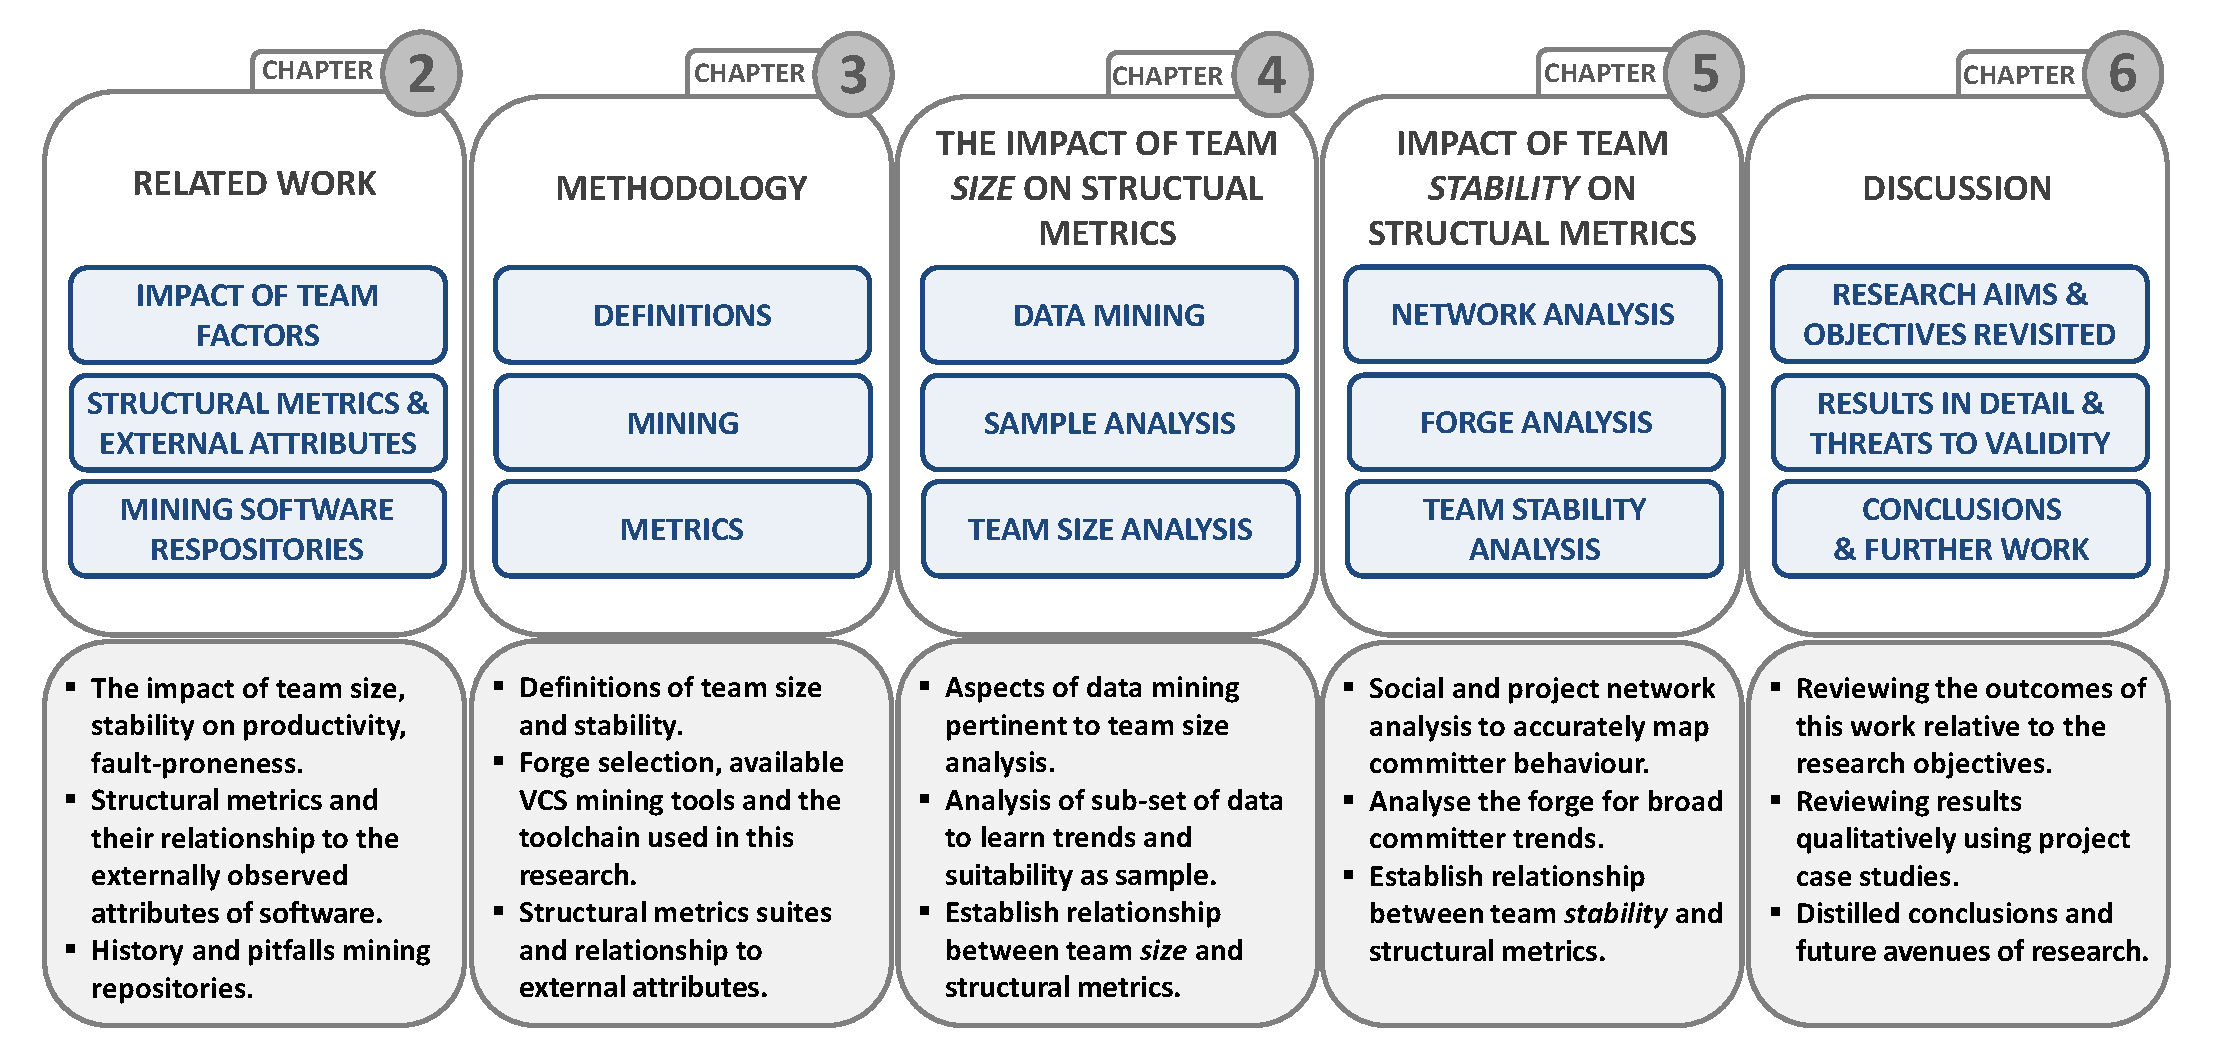
\includegraphics[width=1.4\textwidth]{ThesisOverview.pdf}
\caption[Thesis overview.]{Overview of chapter structure, colour-coded to distinguish mining from analysis.}
\label{fig:ThesisOverview}
\end{figure}
\end{landscape}
